\begin{center}
  \centering 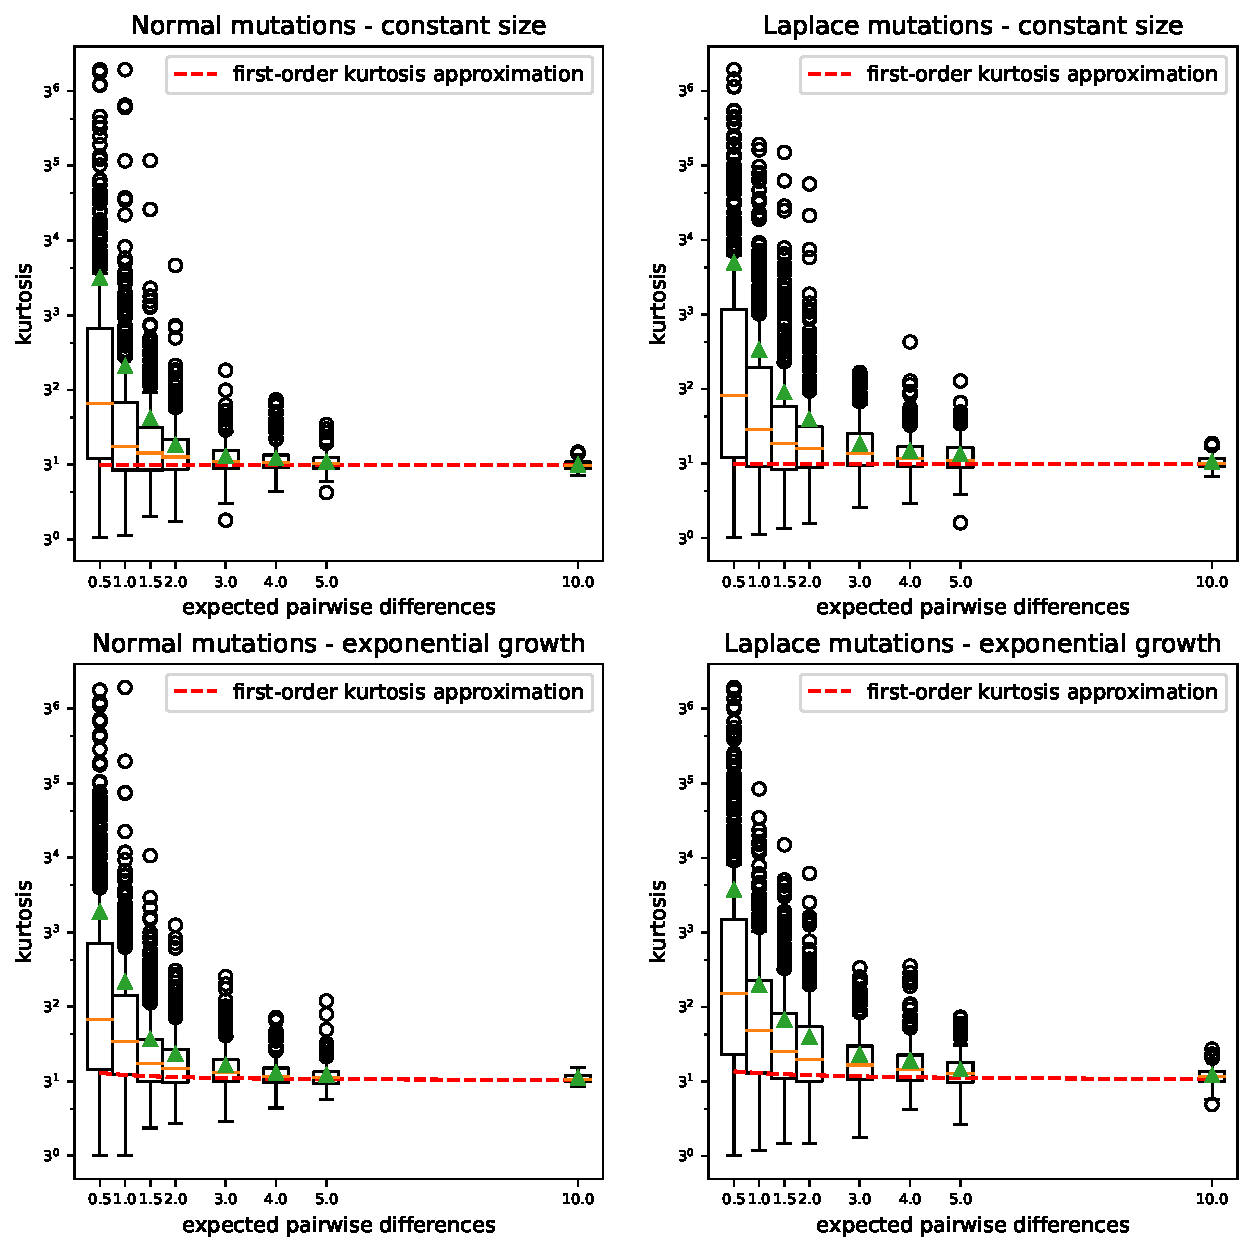
\includegraphics[width=\textwidth]{figures/kurt_sim.pdf}
  \captionof{figure}{The distribution of the population kurtosis under different
    genetic architectures, mutational kernels, and demographies. The genetic
    architecture is varied by changing the expected number of pairwise
    differences at sites affecting the trait. Normal and Laplace distributions
    of mutational effects are compared. A constant size population is compared
    to an exponential growth scenario with growth rate equal to the reciprocal
    of the final effective population size. Green triangles denote the mean
    kurtosis. The dashed red lines give the first order approximation to the
    expected kurtosis given in equation \ref{eq:firstord}.}
  \label{fig:kurtsim}
\end{center}
Entire populations were simulated using msprime \citep{Kelleher2015} and
mutations were assigned effects from a zero-centered normal or Laplace
distribution. The effective population size and mutation rate were kept constant
and the expected number of pairwise difference was increased by increasing the
number of loci affecting the trait.
%%% Local Variables:
%%% TeX-master: "short_report.tex"
%%% End:
